\documentclass{article}
\usepackage[utf8]{inputenc}
\usepackage{graphicx}
\usepackage{hyperref}
\usepackage{dirtytalk}
\usepackage{rotating}	

\usepackage{array}
\newenvironment{conditions}
  {\par\vspace{\abovedisplayskip}\noindent\begin{tabular}{>{$}l<{$} @{${}={}$} l}}
  {\end{tabular}\par\vspace{\belowdisplayskip}}
\hypersetup{
    colorlinks=true,
    linkcolor=blue,
    filecolor=magenta,      
    urlcolor=cyan,
    pdftitle={Overleaf Example},
    pdfpagemode=FullScreen,
    }
\graphicspath{ {./images/} }
\setlength{\parindent}{20pt}
\title{B365 Final Project}
\author{Ting Wei Chou}
\date{April 2022}

\begin{document}

\maketitle

For this final project, I am going to work on H&M Personalized Fashion Recommendations on Kaggle(https://www.kaggle.com/competitions/h-and-m-personalized-fashion-recommendations/data?select=customers.csv).
\section{Problem and data description}
For this project, I am going to come up a product recommendation result based on the data for H&M. H&M is a global clothing brand with online & on-site shopping locations. I am going to find out a way to provide good product recommendations for online shoppers, which means that I am going to provide them the product that online customers desires based on their data. \\
\\
On the Kaggle Database, it includes four data sets: Article.csv, Customer.csv, Sample\_submission.csv and Tractions\_train.csv. Article.csv contains the data for the product; Customer.csv contains the data for customers; Sample\_submission.csv contains a example format for the data output, which we will not use it at the moment; Transaction\_train.csv contains a set of training data for this project.

\subsection{Article.csv - Product Data}
Article.csv contains the detailed information of the products in H&M. This data set contains 25 columns and 105,541 rows. Here are a snapshot for the information of the data:
\\
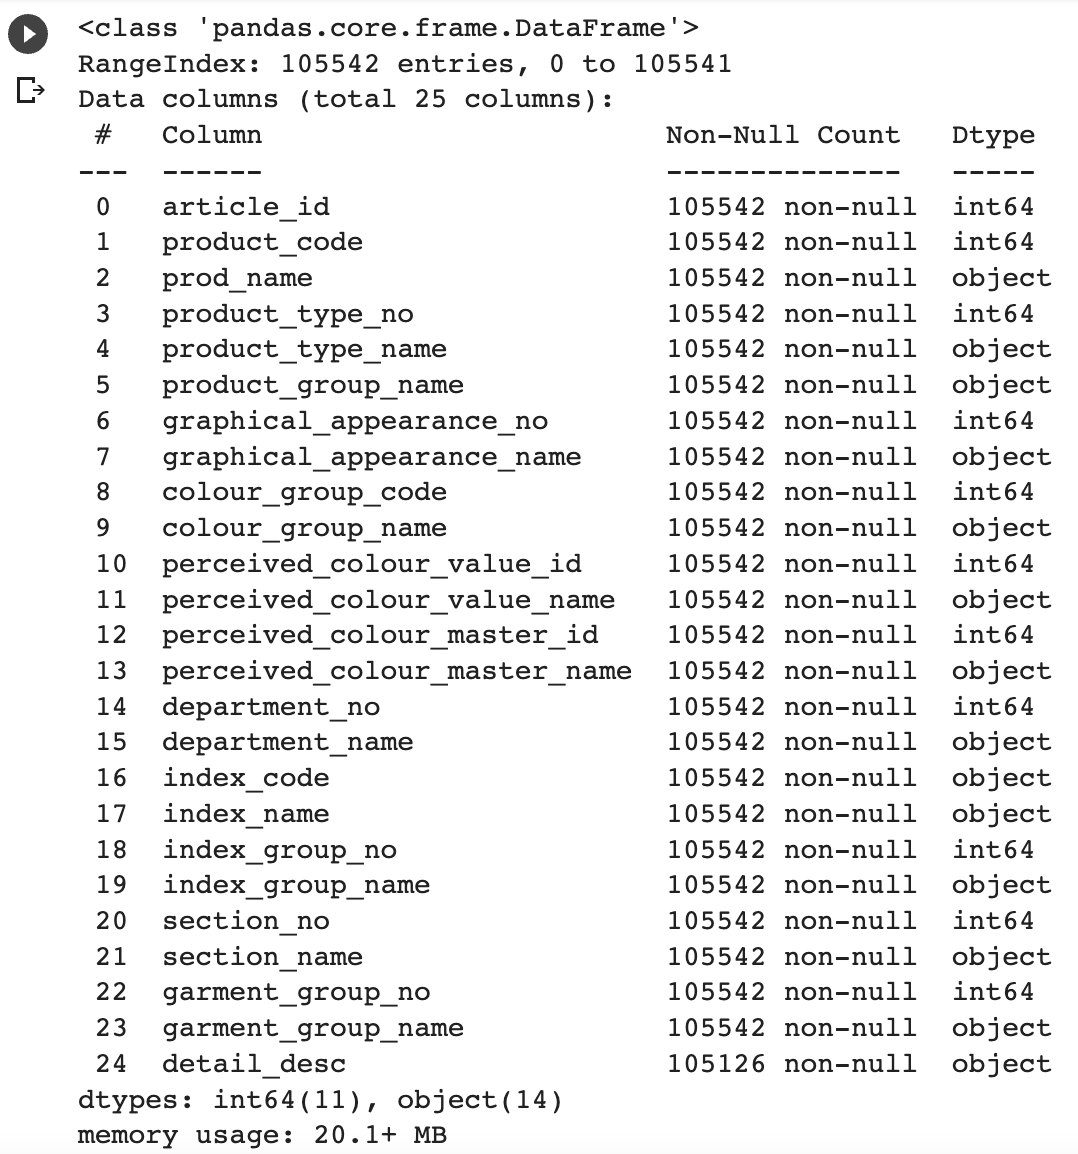
\includegraphics[width=\textwidth]{ProductDataRaw}
\\
We can see that this contains multiple categories of the product, either it's by index, department, graphical appearance etc. This opens a lot of different ways that we can try out while preforming data analysis, allowing us to discover different patterns with the training set.

\subsection{Customer.csv - Customer Data}
\\
Customer.csv contains the metadata of the customer. It contains the customer ID, their age, their zip code (which is encrypted), and information on their membership and activeness. Here is a snapshot of the data structure:
\\
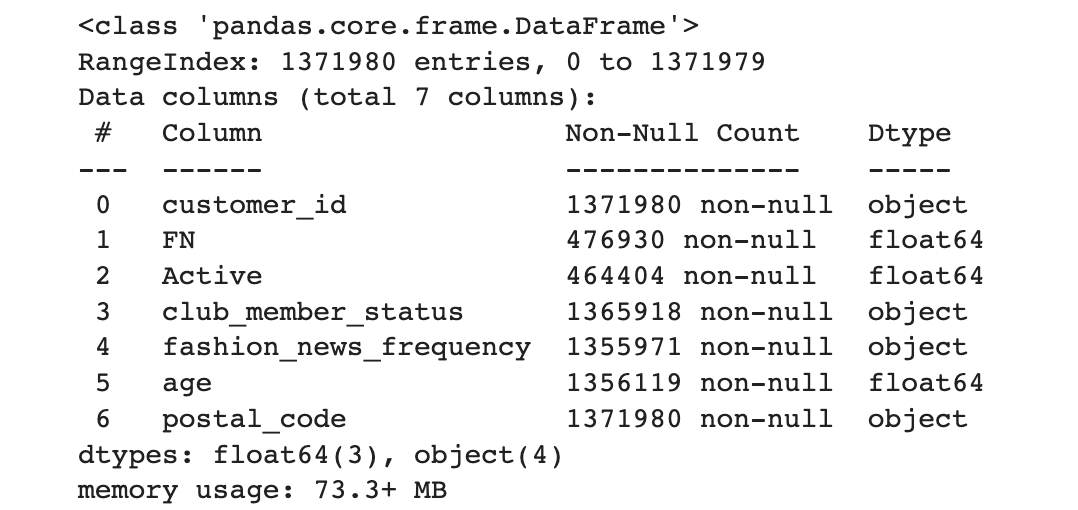
\includegraphics[width=\textwidth]{CustomerDataRaw}
\\
I plan to perform data analysis using their age as a defining factor, and also plan to use postal code but it is unavailable due to encrypted information. I believe that Fashion\_news\_frequency would not be a useful defining factor while processing data since it has nothing related to customer's preference on clothings. 
\\
\subsection{Transaction\_Train.csv - Data Training Set}
\\
This data set is quite self explanatory. It is the training set of the data based on customer.csv and article.csv, and it shows the record of date, customer, product the customer bought, and price. Here is a snapshot of the data structure:
\\
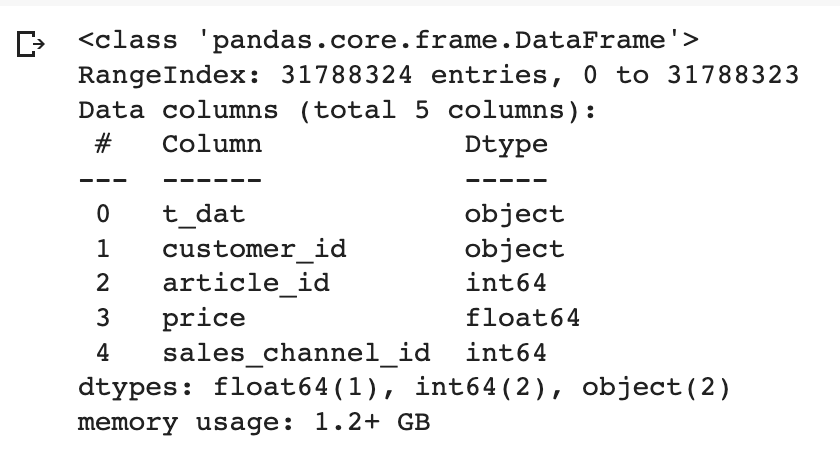
\includegraphics[width=\textwidth]{TrainingDataRaw}
\\
I am going to focus on the customer\_id and article\_id since that's the connection between two data sets, while also the price could also be a determine factor if we have more than one purchase record for each customer.

\section{Data Processing \& Exploratory Data Analysis}
After understanding what each columns in data sets means, lets start to process the data. Since this data is on Kaggle, its already sorted out with given meaning on each columns. I just need to focus on processing missing values and analyzing the data.

\subsection{Data Processing & Analysis - Product}
After putting the dataset into a pandas dataframe, the first thing I did is to find out is there empty data or not. The result returns that there are 416 missing values in the detail\_desc column, which represents the detailed description of the product. I could directly drop the rows with missing data, but I realized that the detail\_desc column is for extra description for products, which would be difficult to analyze it other than looking through it row by row, or string comparisons for each product description. I decide to drop the entire column instead, leaving the rest of the columns all with data and no missing data. Here is the after result:\\
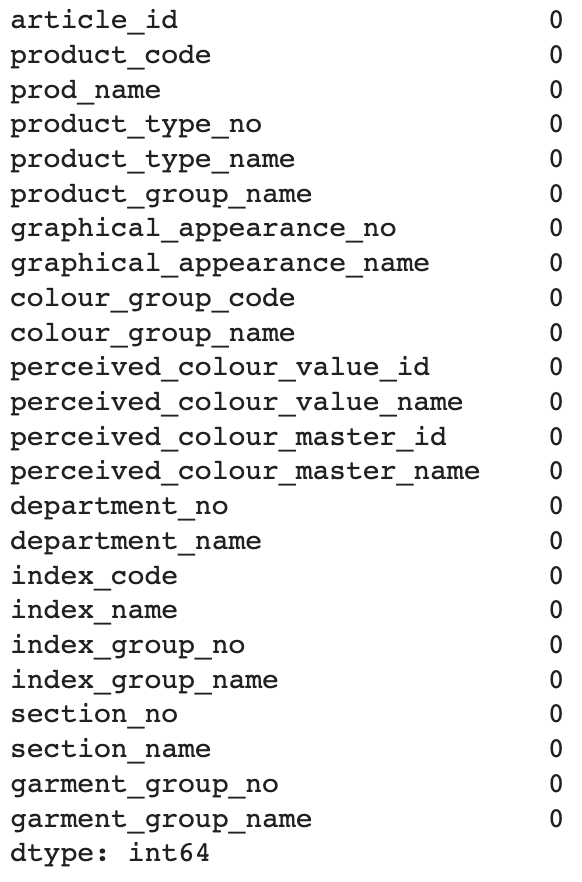
\includegraphics[]{AfterDropProduct}
After cleaning up this data, lets start to visualize it. I started with drawing out some bar chars using different columns, and try to see the relationship between them. Here are two barcharts that uses the index (right) and garment groups(left) as x axis:\\
\includegraphics[width=\textwidth]{barProduct}
\\
Starting by separating with index, which we can see the general distribution of products in H\&M. Ladies wear has the most product, where sports got the lease. This is a good start, where we know the general distribution of the data. Let's move on to process customer's data.

\subsection{Data Processing \& Analysis- Customer}
We start by finding the missing values, as usual. There are multiple missing values, showing below:
\\
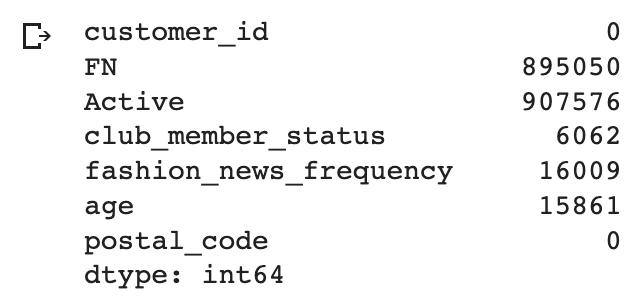
\includegraphics[]{customerisna}
\\
It seems that there are alot of missing values, but if we look closer on what each columns meant, we can see that FN is just a side product of metadata, Active is showing whether the member is active, club\_member\_status shows the account status between active and pre\_create, and fashion\_news\_frequency contains None, Regularly and null. These are not directly related or impact on what customer's taste on product, since they are attributes on account itself, not the customer. The only important column would be age and postal code, which we can categorize and also geo-market. I modified the dataframe to contain only customer\_id, age, and postal code. It leaves the 15861 missing values of age. We could try to fill in the missing data using customer data, but the customer\_id is random and without meaning, so it would be a wrong approach for interpolation. I could use the training data to backtrack the age based on similar purchased product after figuring out the patterns (after algorithms). I dropped the missing values for age right now, and here is the visualized result via histogram:
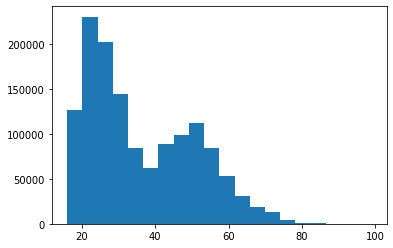
\includegraphics[width=\textwidth]{histcust}
This is the histogram of the age distribution, but in order to cause less bias due to the fact that numbers of bins would affect the visualization result, I also drew a KDE plot. KDE (Kernel Density Estimation) plot visualizes the population density of a continuous variable. In this case, Age.\\
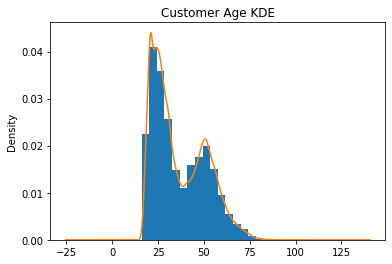
\includegraphics[width=\textwidth]{kdecust}
We can see that most customers from H&M are distributed around age 20 to 30, and also 45 to 55. 

\subsection{Data Processing \& Analysis - Training Data}
There are no missing values in missing data, and we will see more patterns after comparing with our attempt on analyzing in next section. I combined the dataframe with the user's age and also product's information, so I can run the process easier.

\section{Algorithm and Methodology}
In this project, I used three algorithms to come up of a best accurate prediction for user who is on the website: K-means clustering, Random forest and Random Tree prediction.
\subsection{Algorithm}
\subsubsection{K-Means Clustering}
We uses K-Means Clustering in this project to cluster the product by their similarity on category codes, such as section\_name\_catcat\_code and garment\_group\_name\_catcat\_code.\\

K-means clustering requires two inputs, the data set and the number of clusters (k). Here is the pseudo-code of K-means clustering. It will then return K clusters that is grouped by closer distance according to the distance formula. \cite{K-means}: \\
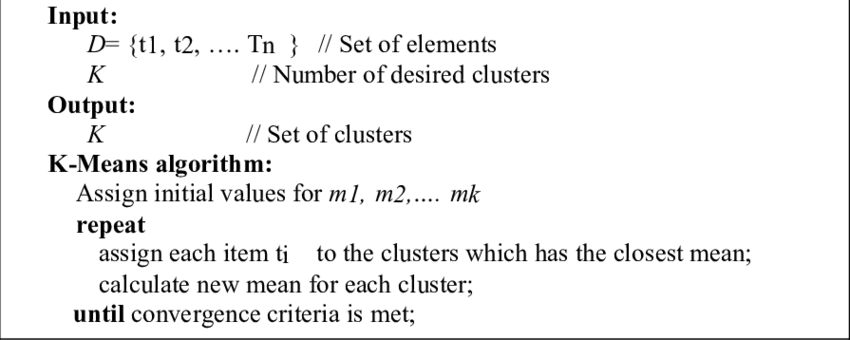
\includegraphics[width=\textwidth]{images/KmeansP.png}

The reason that I choose to use K-means to implement in this project is:
\begin{itemize}
  \item Scales to large database easily
  \item Ability to generalize the cluster to different shapes. 
  \item Definite convergence rate
\end{itemize}
However, there are still downsides of using this algorithms, such as:
\begin{itemize}
  \item Need to choose K manually (number of clusters)
  \item Can only handle numerical data
  \item Clustering outliers (noises).
\end{itemize}
Since we are processing on category numbers for the products, we don't really need to worry on the datatype limitations that K-means brings. I also wrote a function to calculate the optimal K in this data set, which shows the relation between number of clusters and the average sum of inertia (sum of squared distance), and choose the most optimal-point of it.\\
Next, I will talk about how Random Forest and Random Tree Prediction works.

\subsubsection{Random Forest and Random Tree Prediction}
Random Forest is a combined method for classification and regression. Classification in data processing means to take structured / unstructured data and organize it into categories. Regression is a crucial factor where we find out which factor matters the most, which matters the less, and how much should we weight each factor throughout the whole process.\\

As the name implies, random forest is made up of a huge number of individual decision trees that work together as an ensemble. Each tree in the random forest produces a class prediction, and the class with the most votes becomes the prediction of our model. A decision tree is a model that given a state as the node, and different actions as leaves. As different actions leads to more state & more possible actions, the decision tree grows on. Here is an imagery of decision tree \cite{dTree}:\\
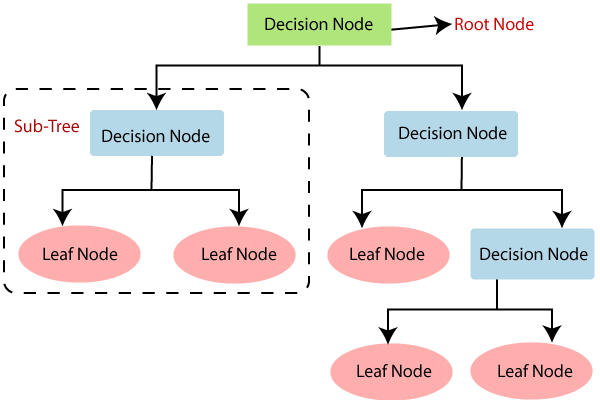
\includegraphics[width=\textwidth]{images/descTree.png}\\
This method handles classification by outputting the class that is selected by most trees; whereas the average prediction of each trees is sent for regression. Here is a simplified flow for Random Forest \cite{randForest}:\\
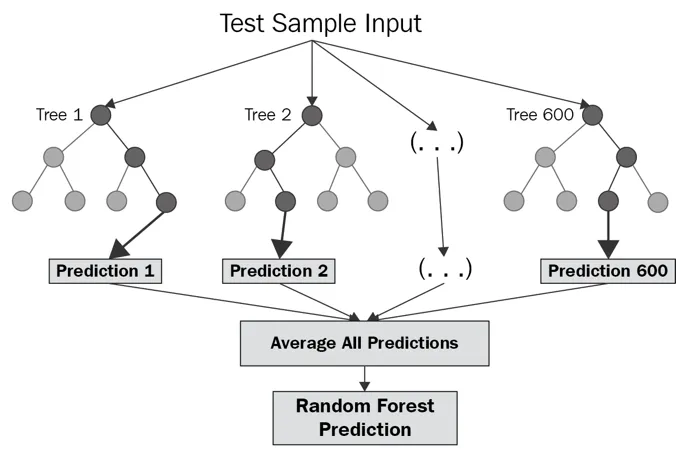
\includegraphics[width=\textwidth]{images/random-forest.png}\\
One of the really interesting thing I learned while understanding Random Forest and why does dumping data into this process can generate accurate result, is the core concept of random forest, the \textbf{wisdom of crowds}. \\
\say{\textbf{A large number of relatively uncorrelated models(trees) operating as a committee will outperform any of the individual constituent models.}}

Just like how it will result if you put thousands of marbles through a \href{https://galtonboard.com/}{Galton Board} and it will result in a Gaussian Distribution, Random Forest takes a bunch of decision trees and come up for the result that would most likely happen. One of the best reason that I choose this model is because the training data are uncorrelated, and it contains a large volume. Uncorrelated models can result with more accurate predictions, since the large amount of decision tree I take will hide the ones that is less accurate, and only show the prediction that is most likely to happen.

After processing the data through Random Forest, I uses random tree prediction to return the processed result.

\subsection{Methodology}
For this project, I am using all the algorithms that I mentioned above to perform data analysis and processing. I will cluster the product data after data process and by categories, and run it among with the training data through classification and regression in the Random Forest method. \\

The precision rate for this method will take in four factors:\\
\begin{itemize}
    \item Mean Absolute Error
    \item Mean Absolute Percentage Error
    \item Root Mean Squared Error
    \item R Square
\end{itemize}\\
The \textbf{Mean Absolute Error} returns the absolute values of the mean of every prediction value errors throughout the data. Here is the formula:\\
\begin{equation} 
MAE = (\frac{1}{n})\sum_{i=1}^{n}\left | y_{i} -  \lambda(x_{i}) \right |\\
\end{equation}
\begin{conditions}
    y(i) & the true target value for test variable x(i)\\
    Lambda(x(i)) & the predicted value for x(i)\\
    n & number of variable tested\\
\end{conditions}
Based on MAE, we can extend to calculate the \textbf{Mean Absolute Percentage Error}, which is more easy to understand since it returns the percentage of error rate instead of error counts. Similar to MAE, the formula is: \\
\begin{equation} 
MAE = (\frac{1}{n})\sum_{i=1}^{n}\frac{\left | y_{i} -  \lambda(x_{i}) \right |}{y_{i}}\\
\end{equation}

\textbf{Root Mean Squared Error} measures the average of the square rooted squared error throughout the data. We can understand as how close is the prediction to the data if we line up the data in a n-dimension space with the prediction data plotted in there.
\begin{equation} 
RMSE = (\frac{1}{n})\sum_{i=1}^{n}\sqrt{( y_{i} -  \lambda(x_{i}))^2}\\
\end{equation}

\textbf{R-Square} returns the percentage of the predicted data through the  model that can explained by the training data. The higher the R-square score is, the better a model fits the dataset. Both RMSE and R-square shows how well a model fits the dataset, where RMSE shows the count and R-square shows the percentage.


\section{Experiments and Results}
\subsection{Experiments}
In order to have a more powerful data processing environment, I installed \href{https://github.com/rapidsai/cudf}{CUDF} that uses GPU in collaborate notebook.\\

I started by taking the transaction data and transform it to a data set that contains \textit{customer\_id, article\_id, count, date (year, month, day)}. Afterwards, since there will be occasions that one customer purchased multiple products throughout the data, I grouped the customers by categorizing each customer and assign them a customer ID. This will simplify the following progress and makes it easier to sort each customers. I then calculate the times bought for each product, and include it to the articles data set.

Moving on, I started to cluster the products in the articles data set by performing K-means clustering. In order to find the optimal K, I took the columns in article data that contains category code (numbers), and run through a loop of K-means to find the optimal K: \\
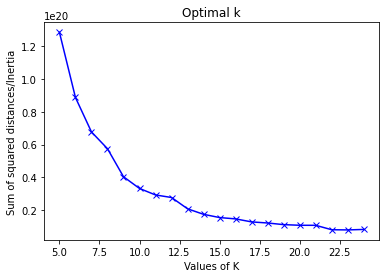
\includegraphics[width=\textwidth]{images/optK.png}
I choose K=12 since its the largest K that still contains a decent sum of distance, and performed K-means clustering on articles with K12. Here is the counts of products in each cluster:\\
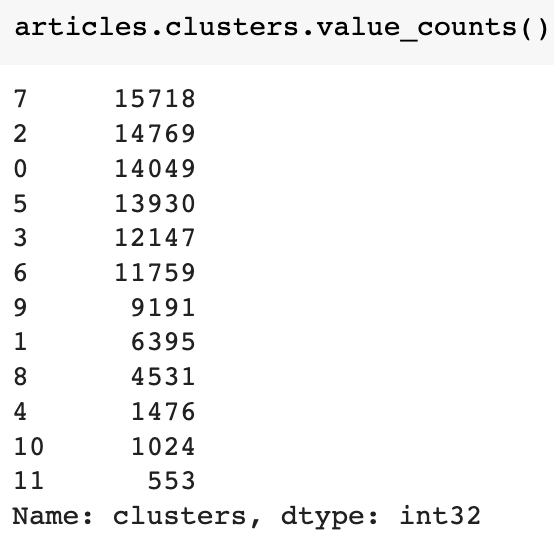
\includegraphics[]{images/12cluster.png}\\
After clustering, I took the list of count columns in articles and the count of each articles and did a regression model with the shape of them. I then run made a random forest model based on that regression, so now I have a model that can perfectly fit through the data set. Afterwards, I ran the Random Decision tree to figure out what will the decision tree represents, which it goes down to a max depth of 22. For show case purpose, here is the representation when I set the max depth to 5:\\
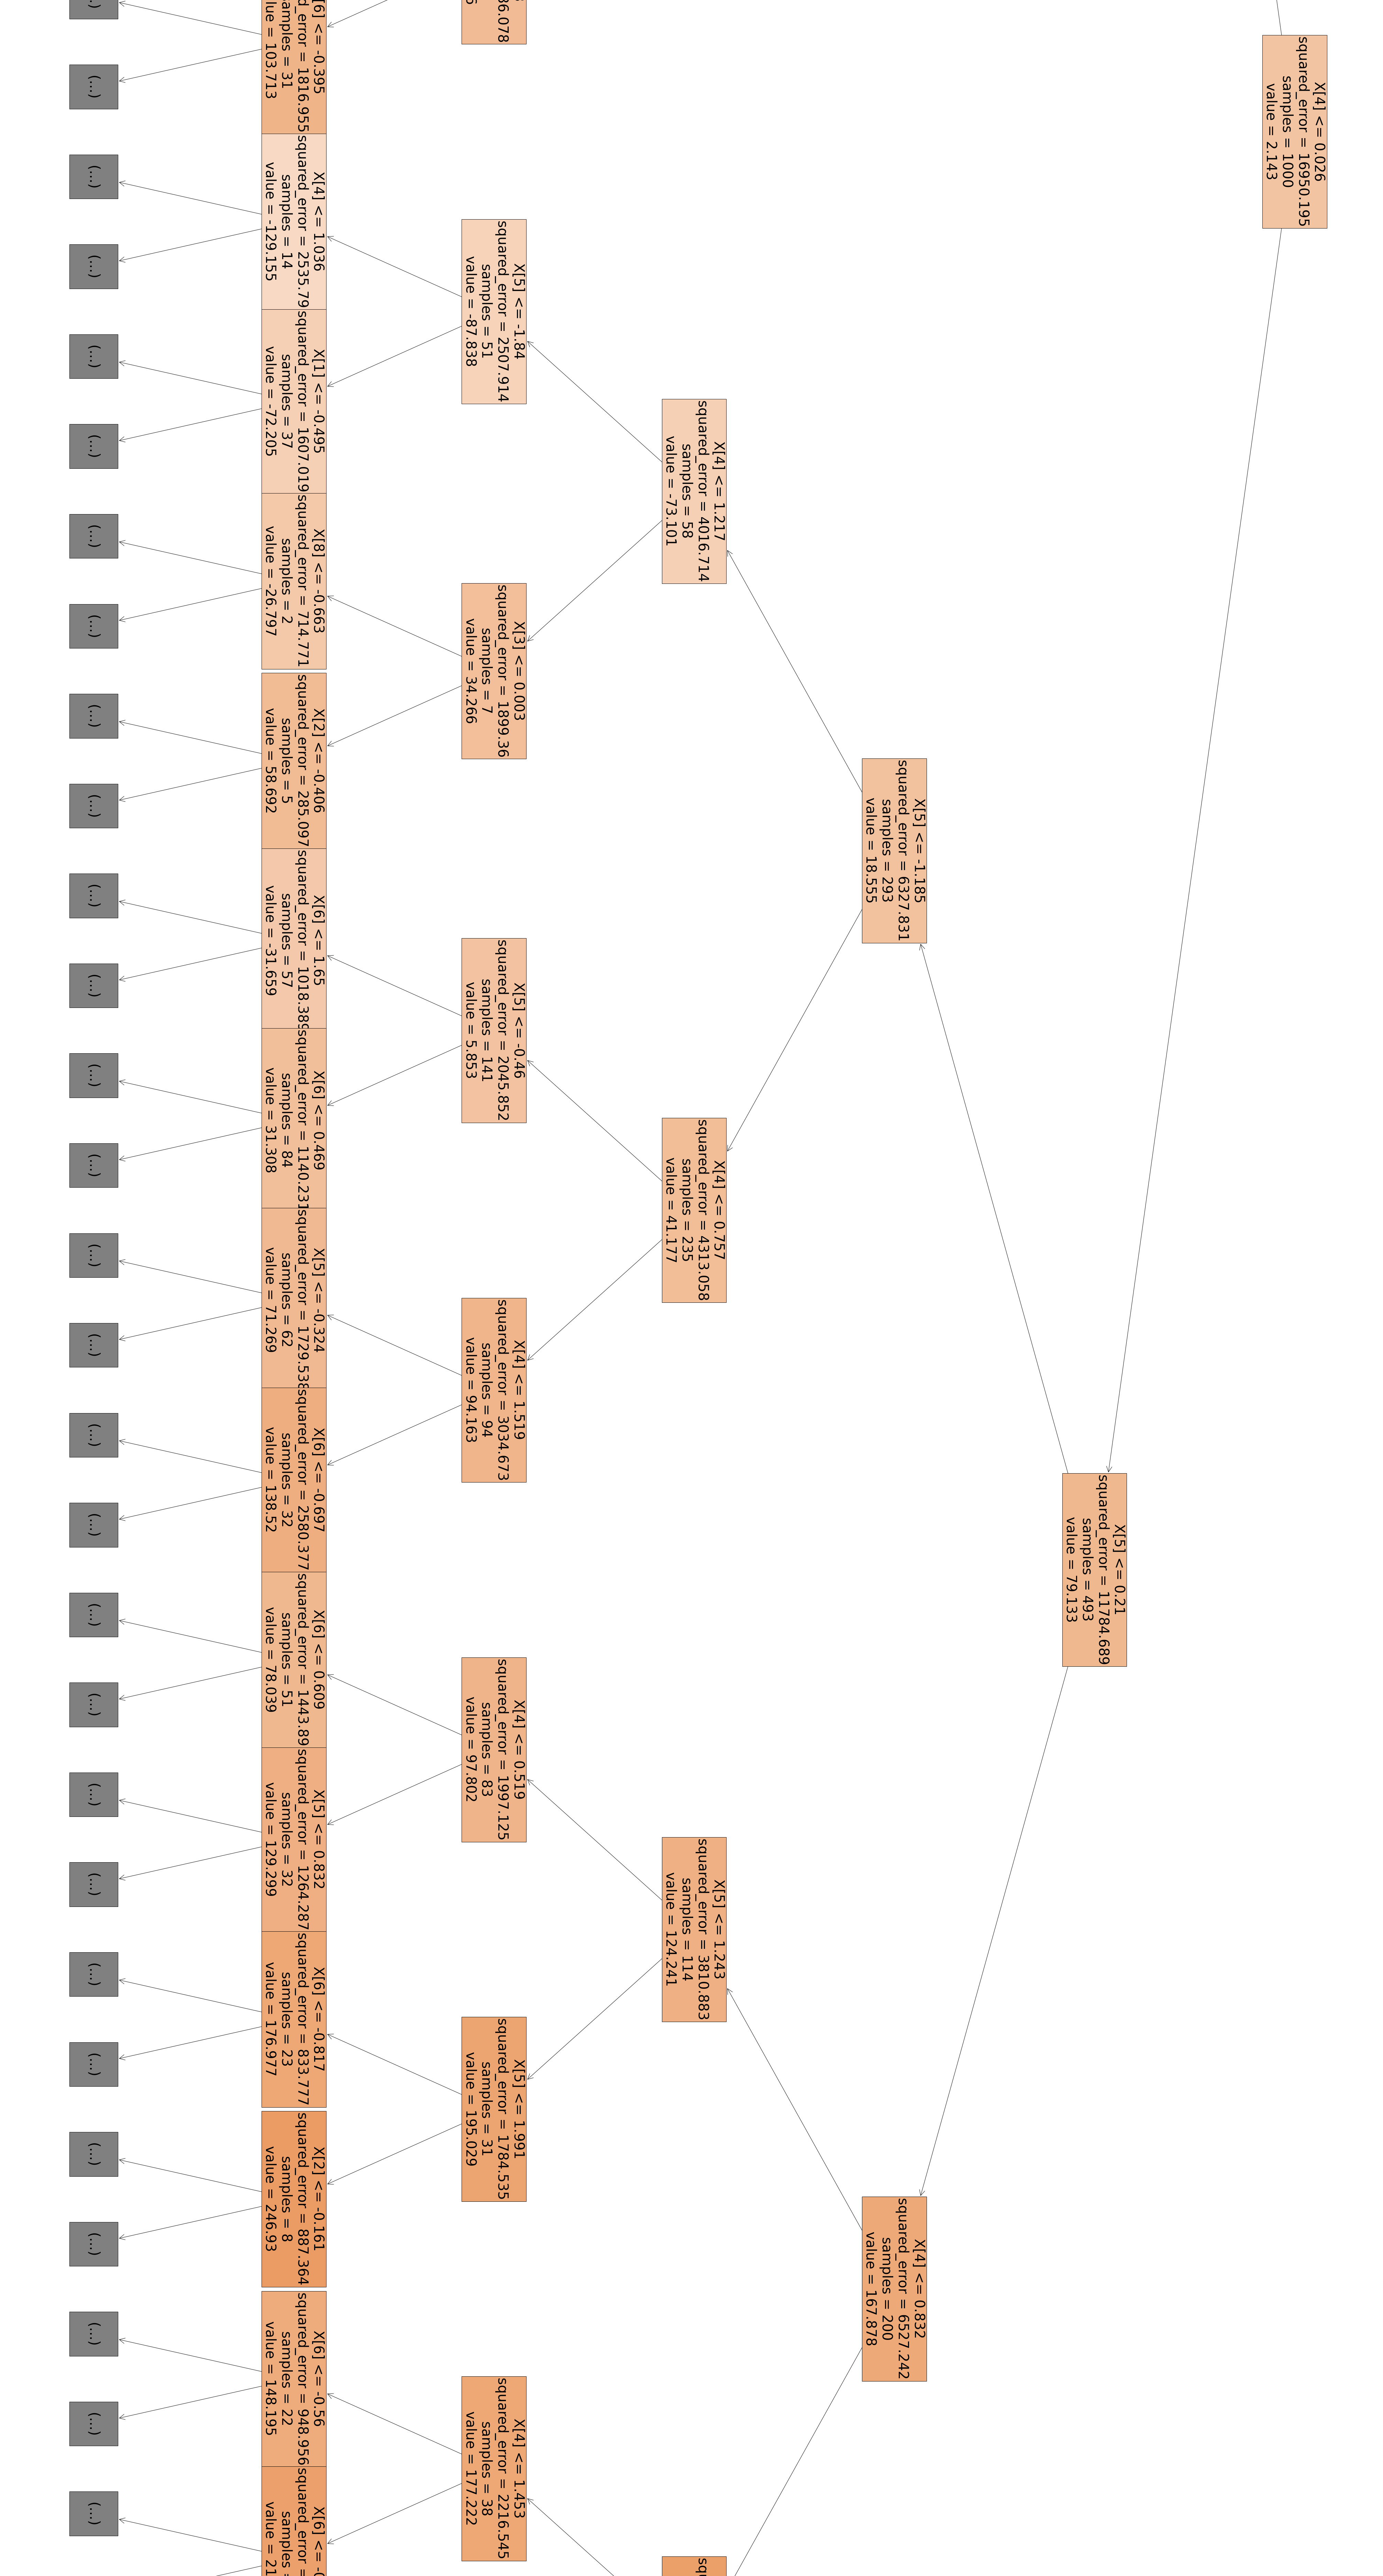
\includegraphics[width=\textwidth]{images/finald5.png}
The uncut and max depth version is attached here \cite{rawTree}. After making sure the models are set, I implement the training data through this model.\\

After building up the model, I calculated the accuracy. I split the training dataset into two, the training data and the testing data. I then run the testing data through my model, and compare the accuracy with the training data. Here are the results of accuracy:\\
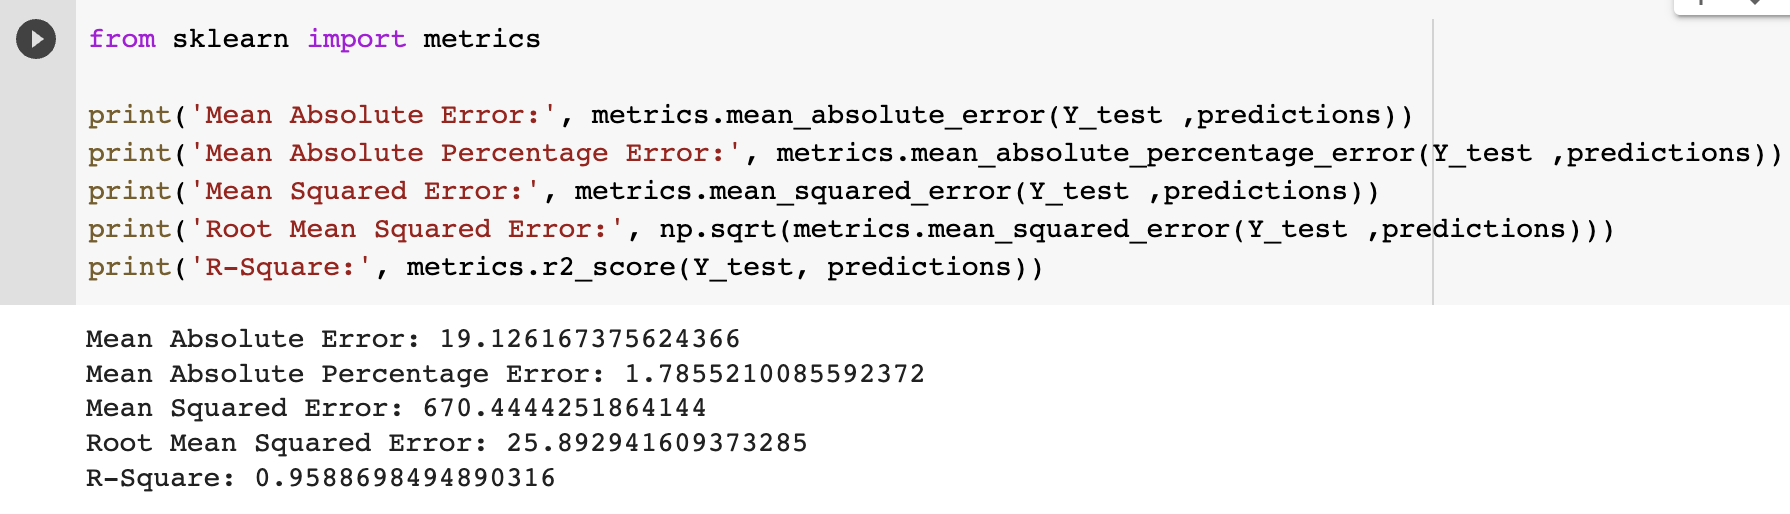
\includegraphics[width=\textwidth]{images/accuracy.png}\\

The Mean Absolute Percentage Error is 1.7855 and R-Squared score is 0.9589. This means that the average percent of error is less than 2 percent, and our model is 95.89 percent similar to the training dataset.


\subsection{Results}
After some quick data transformation, I run the training data through the model. It returns the initial product, and the possible product that the user might buy. I limit the count to 4 in this image, but it could be expanded in the future.\\
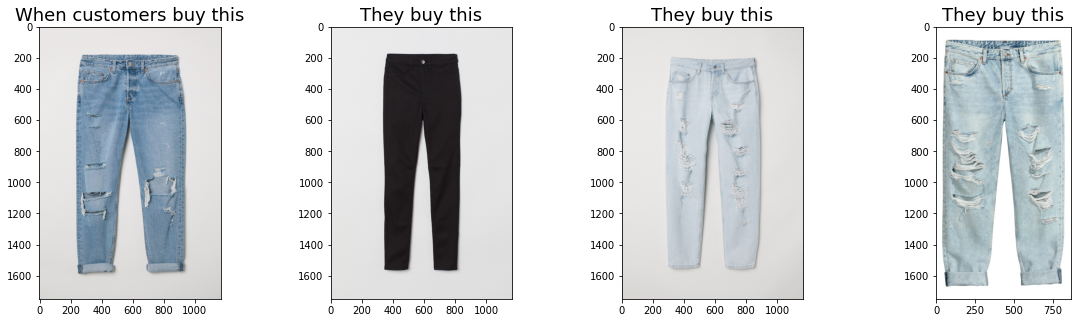
\includegraphics[width=\textwidth]{images/finalprg.png}
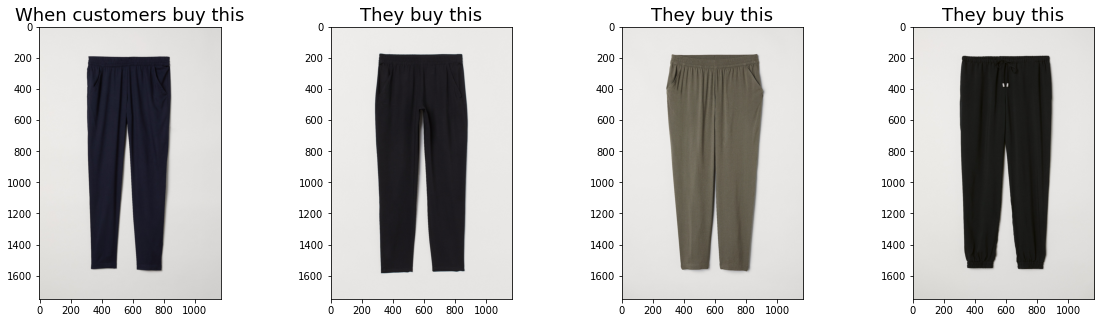
\includegraphics[width=\textwidth]{images/finalprg1.png}
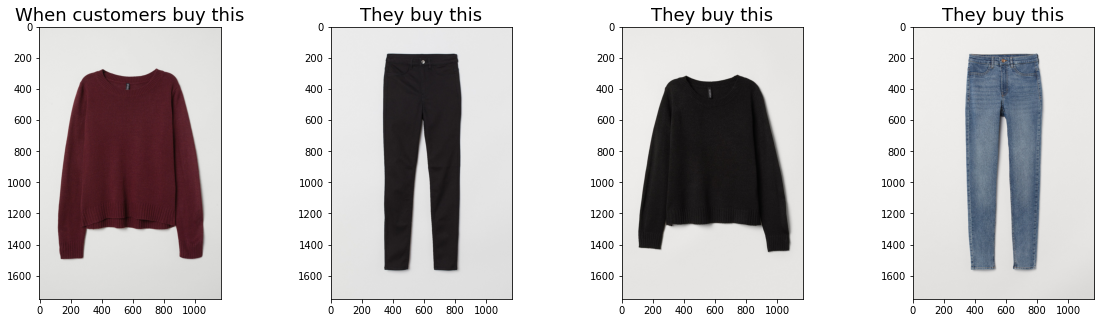
\includegraphics[width=\textwidth]{images/finalprg2.png}
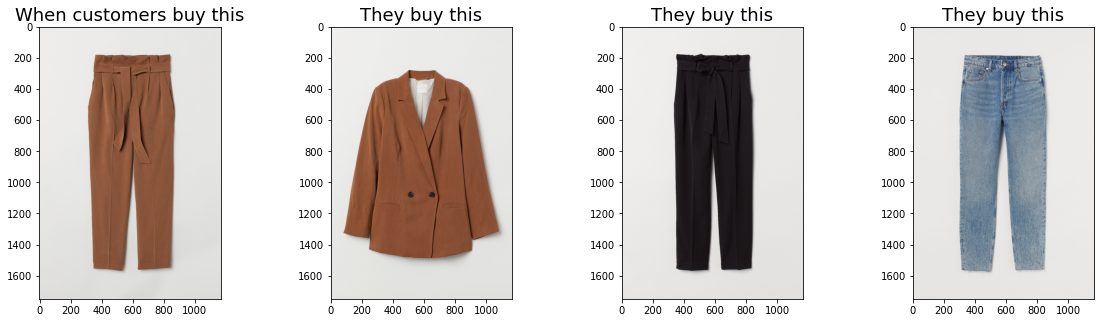
\includegraphics[width=\textwidth]{images/finalprg3.png}
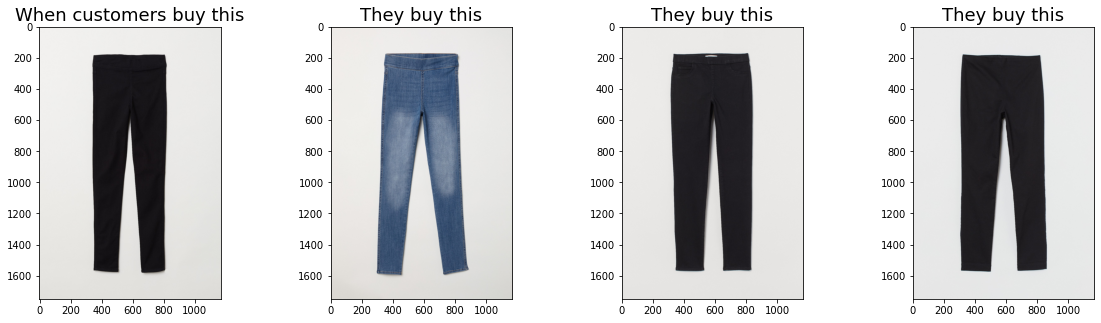
\includegraphics[width=\textwidth]{images/finalprg4.png}
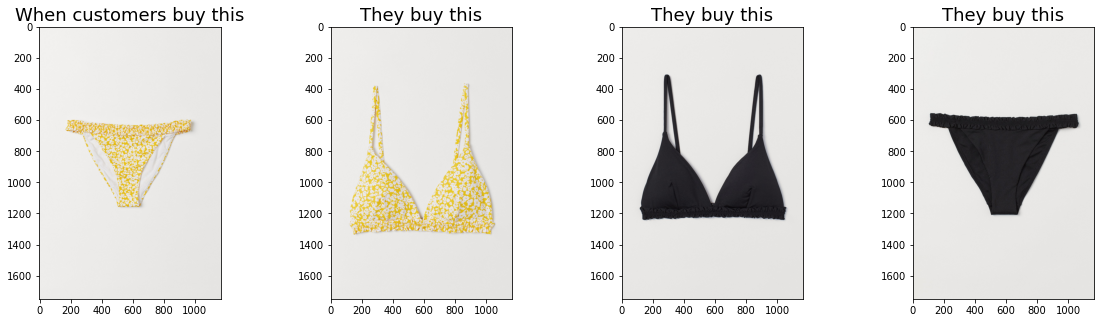
\includegraphics[width=\textwidth]{images/finalprg5.png}
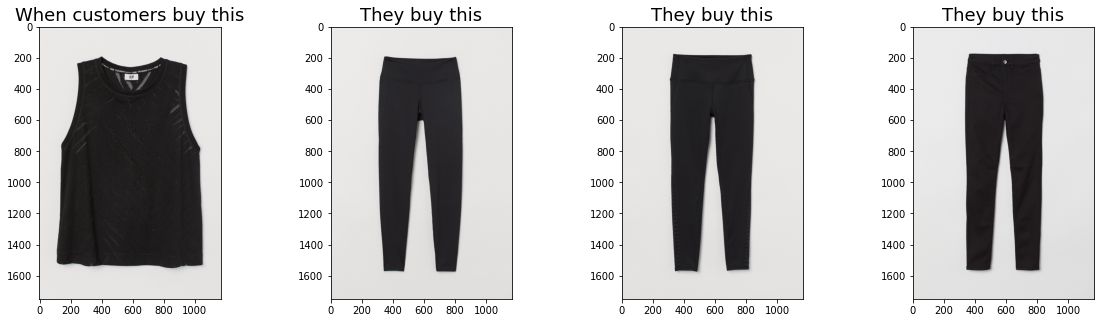
\includegraphics[width=\textwidth]{images/finalprg6.png}
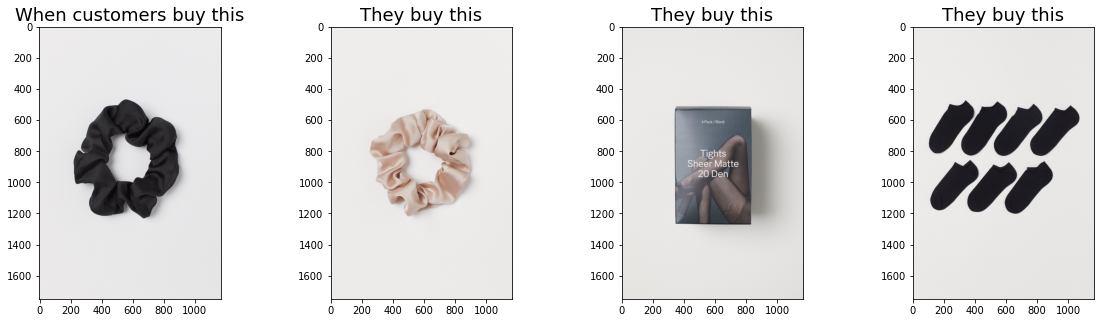
\includegraphics[width=\textwidth]{images/finalprg7.png}
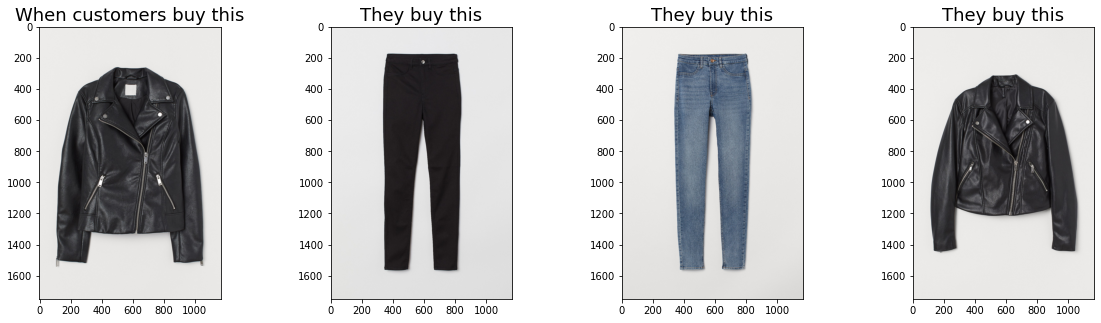
\includegraphics[width=\textwidth]{images/finalprg8.png}
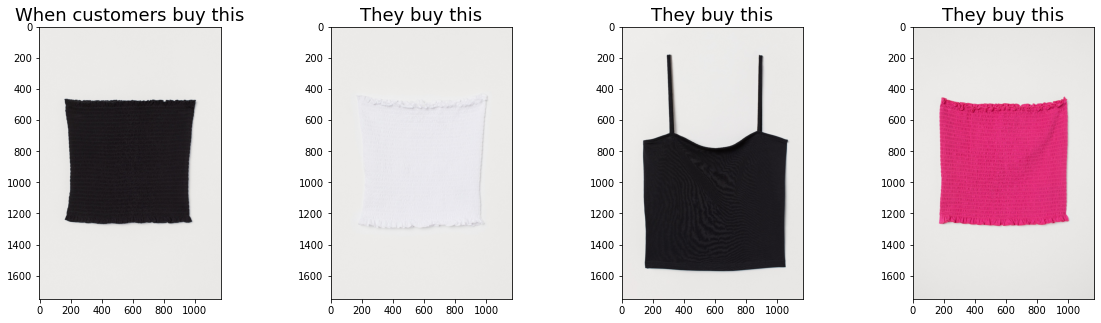
\includegraphics[width=\textwidth]{images/finalprg9.png}
\\
Based on the training model, we filter out the data and come up of the series of suggested product 
\section{Summary and Conclusions}
H&M Group is a family of brands and businesses with 53 online markets and approximately 4,850 stores. Our online store offers shoppers an extensive selection of products to browse through. \\

We aim to develop product recommendations based on data from previous transactions, as well as from customer and product meta data. The available meta data spans from simple data, such as garment type and customer age, to text data from product descriptions, to image data from garment images.\\

So we will explore very important relation which will give us very strong indication of which items were frequently purchased together. Using this information, we can predict which items a customer will buy so we could use this information to increase the probability of make the customer buy it.\\

In this project, we take the training data, customer data and product data, and come up a suggestion set based on previous purchase history by K-means clustering and Random Forest.

The progress is stored inside the collab notebook. I also installed a RAPIDS AI and mini-conda in order to run CUDF in python notebook for faster run time.
\begin{thebibliography}{2}
\bibitem{K-means}
MaxD K-Means: A Clustering Algorithm for Auto-generation of Centroids and Distance of Data Points in Clusters - Scientific Figure on ResearchGate. Available from: https://www.researchgate.net/figure/Pseudo-code-of-the-Lloyds-K-Means-algorithm-K-Means-is-a-simple-algorithm-that-has\_fig1\_278710586 [accessed 1 May, 2022]
\bibitem{dTree}
Machine Learning Decision Tree Classification Algorithm - Javatpoint. (2021). Www.javatpoint.com. https://www.javatpoint.com/machine-learning-decision-tree-classification-algorithm
\bibitem{randForest}
Corporate Finance Institute. (2020, April 27). Random Forest. Corporate Finance Institute; Corporate Finance Institute. https://corporatefinanceinstitute.com/resources/knowledge/other/random-forest/
\bibitem{rawTree}
\includegraphics[width=\textwidth]{images/rawtree.png}
\end{thebibliography}
\end{document}
